\chapter{Computer vision implementation}

Having performed a review of literature relevant to the project, it was time to actually build the tracking system.

This chapter describes the steps required to establish a complete computer-vision workflow. Unlike other chapters in this report, it is likely that the software presented here will quickly become outdated - multiple computer vision frameworks are competing for market attention, and changing a lot while doing so \cite{website:comparison_deep_learning_software}. In addition, neural accelerator technology is in its infancy and likely to improve a lot in the coming years. Thus, the section is presented as a general methodology which tries to be independent of framework and branding where possible.

Following this, the actual implementation of the computer vision system is discussed along with some short tests on its performance.

%It should be noted that a lot of mistakes were made in this part of the project - these won't be discussed.

\section{Workstation setup and testing}
Three independent computers were used as part of the complete computer vision workflow - a mid-range GPU-equipped computer to prototype and train neural networks, a regular laptop to test and compile a trained neural network and an small embedded computer which uses the neural accelerator for inferencing.

One software package common among all three computer was git \cite{git}, which was used extensively to keep the files on all three computers synchronized.

\subsection{Setting up a computer for training}
Depending on the selection of computer vision/deep learning framework and the operating system on which it is installed, setting up a computer to train neural networks can range from trivial to extremely difficult. However, there are some commonalities amongst the popular frameworks.

The first step is usually to install CUDA, a GPU-acceleration software developed by NVIDIA for their GPUs \cite{nvidia_cuda}. At the time of writing, most frameworks simply don't support AMD GPUs. Next, install cuDNN, NVIDIA software specifically aimed at increasing performance for deep neural networks \cite{nvidia_cudnn} on their GPUs.

If needed for the deep learning framework, install an appropriate version of python \cite{python}.

Finally, the framework itself should be installed. In this project, three frameworks were tested on Windows.

The first two were TensorFlow and Keras. These are installed using pip, pythons built in package manager. The installation is done by entering the command,\\
\pyth{python -m pip install keras tensorflow-gpu}.

The last package was Caffe. Installation on Windows is difficult due to a lack of support for the OS, and wasn't accomplished during the course of the project.

It should be noted that, if the network will simply be fine-tuned (ie, the network was already trained on a similar dataset and requires minimal further training) then one might actually get away with training the model on a fast CPU.


\subsection{Setting up a computer for testing and compiling}
Most simple tests were run on an easily accessible computer. If using the Movidius NCS, this computer must run a Ubuntu 16.04 as it is the only non-Raspbian desktop OS the Movidius SDK officially supports \cite{website:movidius_install}. Movidius software barely works as is, so it is not recommended to push things even further by messing around with any other OS.

One option is to run Ubuntu on a virtual machine, such as Oracle VirtualBox. If you do this, don't bother trying to make it work with the NCS hardware through the VM - it can be quite tricky getting the drivers to work. Instead, trust that the compiled network will perform as well on the NCS as it does in the uncompiled framework-specific format and save yourself a lot of time.

Next, install the Movidus SDK, as described in the documentation \cite{website:movidius_install}. Despite what the documentation suggests, there isn't a need to \pyth{make} all the examples - this can take a couple hours, use a lot of disk space and not help at all.

After this, the previously trained neural network should be compiled to the Movidius-specific graph format using the \pyth{mvNCCompile} command. If it fails, it is likely that the network has an operation which isn't supported by the Movidius software. To this end it is highly recommended to check whether the operations used in the neural network are supported by Movidius for that particular frame.

If the Movidius SDK installation process has not already done so, it is recommended to install the deep learning framework that will be used. This enables the user to debug their neural network without having access to the inference computer.


\subsection{Setting up a computer for inferencing}
A Raspberry Pi was chosen as the embedded computer that would interface with the neural accelerator. An SSH terminal was used to access it. In order to get it ready for the final platform, some packages needed to be installed - a list of the most relevant python packages not included in a default python installation is as follows:

\begin{itemize}
	\item \pyth{numpy}: a package for fast numerical computing.
	\item \pyth{picamera}: a package to facilitate the use of the Pi Camera module.
	\item \pyth{matplotlib}: a popular plotting library.
	\item \pyth{PIL}: an fast library useful for working with images.
\end{itemize}

These are easily installed by entering the following command in a terminal:\\
\pyth{python -m pip install numpy picamera matplotlib PIL}

Interestingly, it is not actually necessary to install any deep learning framework on the Raspberry Pi. Neither is it necessary to install \pyth{opencv} or even the full Movidius SDK if the neural network has already been compiled to a graph file. Knowing this can save you an absolutely incredible amount of time, as these programs can be incredibly time consuming and frustrating to install. For instance, installing the full Movidius SDK on the Raspberry Pi requires upwards of 10 hours and is prone to failing at almost any point in this installation.

Thus, it is \emph{highly} recommended to instead skip all of these potential issues and rather just install the Movidius SDK in API-only mode \cite{movidius_api_only}. This doesn't take long and is not prone to failure.

Python notebooks were used for all actual programming. In this project, the main advantage to using notebooks was the fact that the notebook server could be port-forwarded to the main development PC, allowing for far easier plotting and visualisation than would be possible using a simpler IDE in an SSH terminal. Note that was important that the code ran on the Raspberry Pi itself to access its hardware, and connect the Pi to an external display would not be ideal as its GPU was needed for other computation.


\section{Selection of computer vision framework}
At the time of writing, the Movidius NCS only supports the TensorFlow and Caffe machine learning frameworks \cite{website:movidius_install}. Based largely on its popularity and ease of use, TensorFlow was chosen as the architecture which would be used for the project \cite{website:tensorflow_popularity}. However, TensorFlow is quite low-level and provides fairly slow and inconvenient methods of model creation, training and testing. It certainly has advantages but ease of development is not one of them.

To combat this, another option is to instead use Keras, a deep learning library which provides a far more intuitive interface. It allows the user to specify which backend they'd like to use for the actual number crunching. Among other options, one of the available backends is TensorFlow. The popularity of Keras has grown to such an extent TensorFlow has incorporated it as an official API.

The plan was then to retrain a neural network (possibly after modifying it) using Keras, export the model architecture and weights in TensorFlow format, and then compile it down to the Movidius NCS graph format. The hypothesis was that while researchers often aim to create neural networks which can classify more and more types of classes at once, this project only required up to three: cheetahs, humans and dogs. This meant that useless parts of the network (neurons which never fire as they aren't needed) could potentially be removed \cite{molchanov2016pruning}. This process is known as 'pruning', and can significantly decrease inference time.

However, after far, far too much frustration, it was discovered that the support for each framework was far from equal. Networks created in TensorFlow quite consistently failed to compile. After examining the Movidius documentation more closely, it was discovered that the number of operations supported for TensorFlow was simply far smaller than the number supported for Caffe. For instance, the TensorFlow \pyth{concat} operation doesn't appear on the list of compilable operations. This left Caffe as the only other available framework.

\section{Selection of CNN architecture}
By this stage, the work spent on object detection had exceeded time estimates and was threatening to compromise the time available for the other components in the system. In addition, Caffe has extremely poor support for Windows machines and no there were no dedicated GPU-enabled Linux PC was available for use as a neural network training machine. For these reasons, it was decided the an unmodified pretrained Caffe model would be used.

%https://github.com/movidius/ncappzoo/tree/master/caffe
In order to mitigate further risk of a model not working correctly on the NCS, only architectures with official support from Movidius were considered. At the time, this narrowed the choice down to a single option: SSD MobileNet, the combination of MobileNet and SSD, two independently designed neural network architectures.

MobileNet is a class of image classifiers designed by researchers at Google \cite{arXiv:1704.04861}. Since it was designed for mobile devices, it trades some classification accuracy for performance. However, the architecture is remarkable in that the performance increase is usually significant while the classification accuracy decrease is not. It acts a feature extractor in this particular model.

SSD (short for Single Shot MultiBox Detector) is a an object detector \cite{arXiv:1512.02325}. When used with another network as a feature detector, it takes in features, scales them to a variety of sizes and finally, after some more processing, outputs a vector which embeds information on the number of objects found, the predicted class for each object, pixel coordinates of the bounding box around each object and a number from 0 to 1 which represents the confidence in the network's prediction. Hence, the name - a single pass through the network resulting in the detection and boxes of multiple objects.

As a backup, another option would have been to perform the sliding window technique using an image classifier. There could be merit to this: a clever algorithm might first search parts of the image where it expects to find the object, reducing the overall computational requirements.


\section{Implementation of computer vision system}
Once all required software packages were installed, the next step was to start integrating the various components in the computer vision pipeline.

\subsection{The Raspberry Pi camera}
For the sake of convenience and low latency imaging, it was decided that a Raspberry Pi v2 camera module would be used to provide a stream of photos for the CNN. The camera plugs into a Raspberry Pi using a flat ribbon cable, as shown in Figure~\ref{fig:r_pi_camera}.

\begin{figure}[h!]
  \centering
  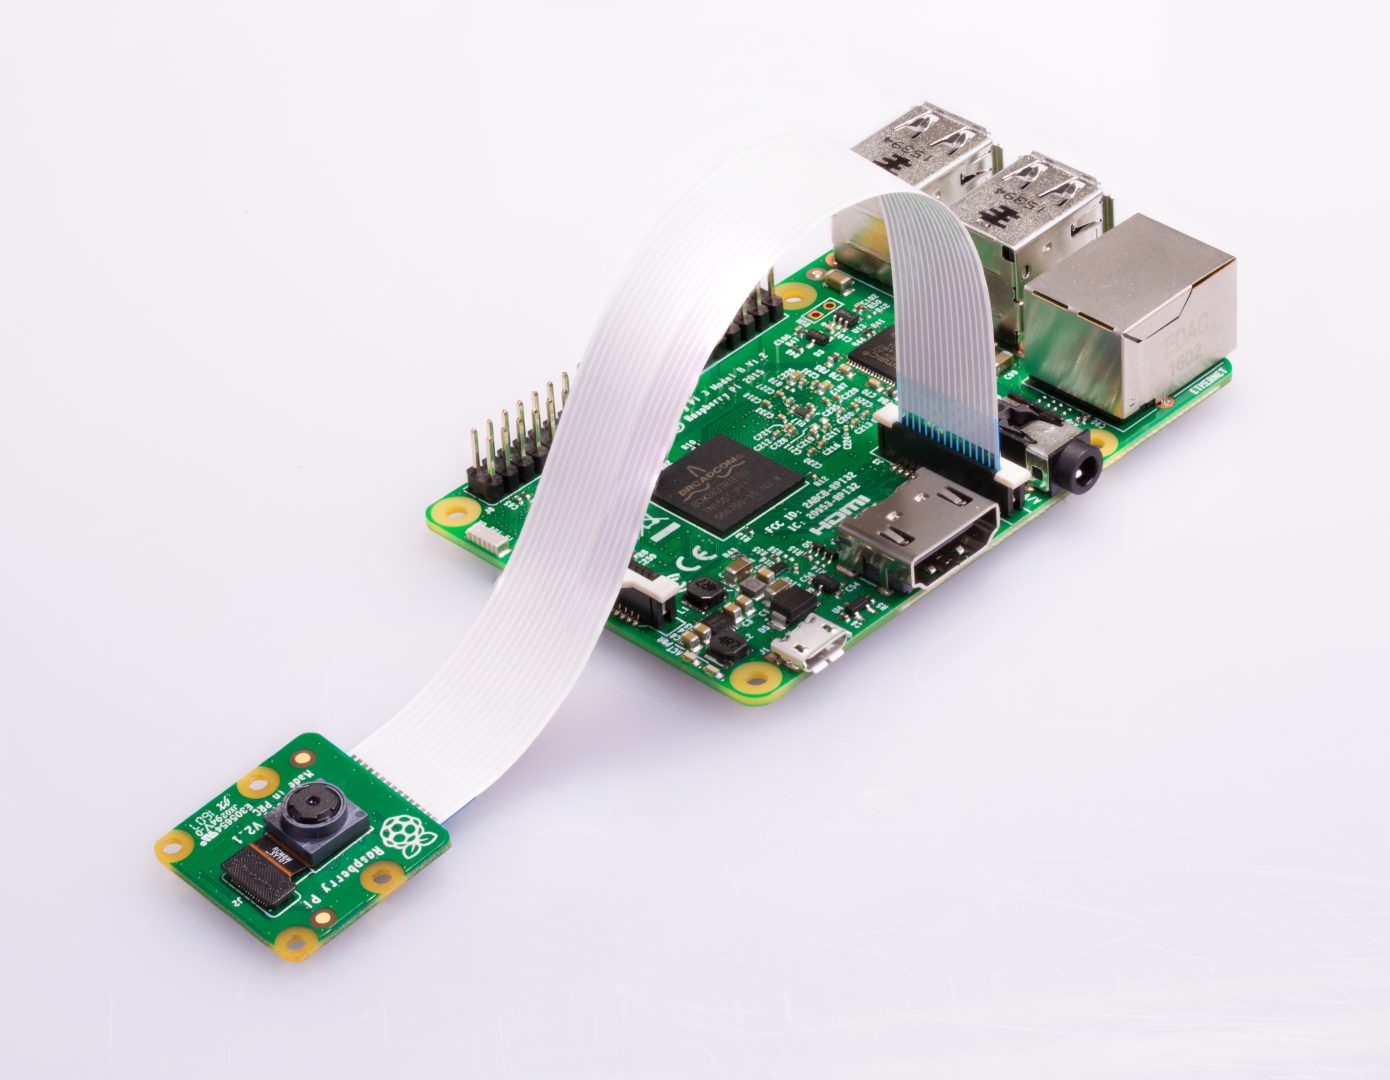
\includegraphics[width=0.5\textwidth]{methodology/r_pi_camera}
  \caption{\label{fig:r_pi_camera}A photo of a Raspberry Pi connect to a Raspberry Pi camera module.}
\end{figure}

An alternative would be to attempt to stream from the GoPro cameras themselves, but this would result in a higher latency as the photos have to be transferred via WiFi and would not use the Pi's built in hardware encoding \cite{website:gopro_to_rpi, website:gopro_to_rpi2}.

As described in the excellent \pyth{picamera} module documentation \cite{website:picamera_hardware}, one must be careful about selecting a sensor mode and camera resolution which makes use of the full FOV available (62.2\textdegree $\ \times$ 48.8\textdegree). Lower resolutions and fast sensor modes tend to take a simple crop of the centre of the image (reducing the FOV) instead of taking a full photo and resizing it. The price paid for this is latency - the higher the resolution, the more data flows through the pipeline and computation must be done.

A resolution of \pyth{1640 x 1232} maximised the FOV. Since the Pi Cameras sensor resolution is \pyth{3280 x 2464}, it uses 2$\times$2 binning to easily achieve this downscaling. Next, the Pis GPU was used to easily resize the image down to \pyth{320 x 304} - only a few resolutions are support by the library and this one was close to the resolution typically used by CNNs, so further resizing on the Pis CPU would require minimal processing time.

Finally, the video port was used to take photos instead of the camera. This was done to decrease latency - while both the video port and still port constantly send photos down the ribbon cable to the pi, using the video port results in less anti-noise post-processing (and thus lower latency).

%As is normal in Python, once the exact problem had been understood, the solution in code was relatively straightforward. The following code is enough to set up the pipeline mentioned thus far: \\ \\ \\ \\

%\begin{python}
%with picamera.PiCamera(resolution=(1640, 1232),
%                       framerate=40,
%                       sensor_mode=5) as camera:
%     # (320, 304) is closest to neural network input of (300,300)
%    frame = picamera.array.PiRGBArray(camera,
%                                      size=(320, 304))
%    # use GPU for resizing - will resize to nn_shape later
%    cont_capture = camera.capture_continuous(frame, 'rgb',
%                                             resize=(320, 304),
%                                             use_video_port=True)
%\end{python}

%After this, a simple function call of \pyth{next(cont_capture)} would fetch the latest frame from the continuous stream of photos, perform some post-processing and then place it in the \pyth{frame} buffer, where it could be accessed using \pyth{frame.array}.

\subsection{Compiling a trained neural network}
A trained SSD MobileNet was found on GitHub user chuanqi305's \href{https://github.com/chuanqi305/MobileNet-SSD}{online git repository} \cite{website:chuanqi305_nn_github}. It has an input dimension of $300 \times 300 \times 3$, and was largely trained on MS-COCO before being fine-tuned on VOC0712 (MS-COCO and VOC0712 are two large, freely available datasets \cite{website:mscoco_dataset, website:voc2012_dataset}). It was trained to predict make predictions for 20 classes, including 'person', 'dog' and 'cat'. The reason for choosing a network which predicted these classes, was because tests would be done on (easily accessible) humans and dogs. In addition, if the network was to be retrained to detect cheetahs, starting from detecting cats or dogs might help decrease training time and the amount of data required.

After confirming that the license for usage of the model is permissive, it was downloaded and then compiled on a windows laptop running an Ubuntu VM with the full Movidius SDK installed, using the \pyth{mvNCCompile} command. The graph file was then transferred to the Raspberry Pi via an ssh terminal.

Using Movidius code from tutorials as a starting point, the graph file was uploaded to the NCS. The camera module presented above was then used to take a photo and store it as an array of unsigned 8-bit integers (integers from 0 to 255).

The CNN used required some preprocessing before an image could be passed in as an input. Specifically, the images should be represented as an array of floats with a mean of 0 and a range of $(-1, +1)$. This was done using the calculation,%\\ \\

\begin{python}
mean = (127.5, 127.5, 127.5)  # 3 colour channels, 255/2 == 127.5
scale = 1/127.5
preprocessed_img = (img - np.float32(mean)) * np.float32(scale)
\end{python}

Pre-processed images were then sent to the NCS, which passed them through the CNN in a time of about 80 ms. The serialized output of SSD network was then decoded into a python dictionary which contained easy to manage information about the objects in the frame.

\section{Testing the computer vision model}
The next step was to test the data pipeline created thus far. The main issues being tested were,

\begin{enumerate}
\item The general classification accuracy of of the network,
\item The extent to which the predicted position overlaps with the actual position,
\item How blurry/dark/out of focus the image can be before the network stops working, and finally,
\item The inference time of the network, with and without the NCS.
\end{enumerate}

Code to redo these tests can be found on the authors \href{https://github.com/alknemeyer/EEE4022S-Thesis-Project/blob/master/Final%20code/tests.ipynb}{GitHub repository}.


\subsection{Accuracy of the predictions}

The setup was tested by passing photos through the neural network, and then superimposing the predicted bounding box output onto the image along with a text description of the predicted class. A measure of confidence (written as a percentage by convention, but not actually a statistical measure) was also added to show how trustworthy the prediction was.

First, a photo of the author's dog was tested. The network correctly predicted 'dog' with a high confidence measure of 99\%. This is shown in Figure~\ref{fig:box_around_blossom}.

\begin{figure}[h!]
  \centering
  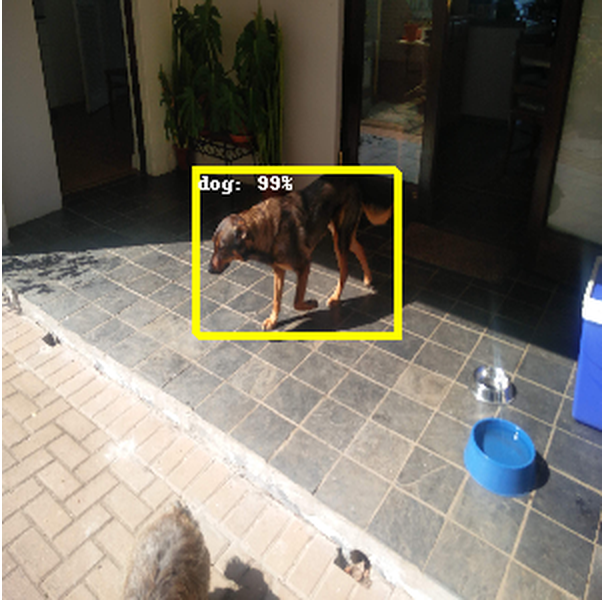
\includegraphics[width=0.7\textwidth]{methodology/box_around_blossom}
  \caption{\label{fig:box_around_blossom}A photo of the authors dog, correctly predicted with 99\% confidence.}
\end{figure}

Next, three images of the author were tested. They are shown in Figures~\ref{fig:box_around_me_crouching}, \ref{fig:box_around_me_running} and Figure~\ref{fig:box_around_people_hard}.

\begin{figure}[h!]
    \centering
    \subfloat[][A photo of the author while crouching, correctly predicted with 88\% confidence.]{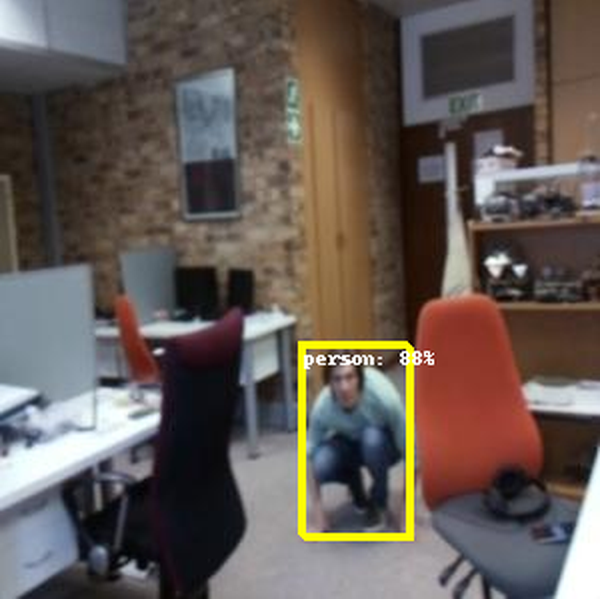
\includegraphics[width=0.48\linewidth]{methodology/box_around_me_crouching}\label{fig:box_around_me_crouching}}
	\quad
    \subfloat[][A photo of the author while running, correctly predicted with 96\% confidence.]{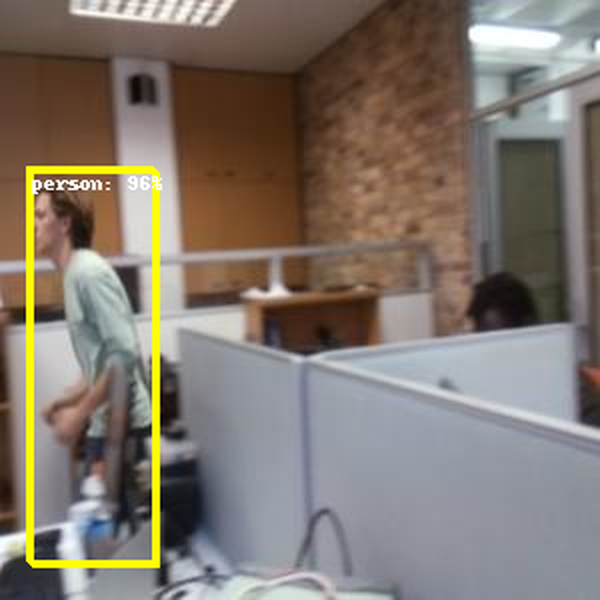
\includegraphics[width=0.48\linewidth]{methodology/box_around_me_running}\label{fig:box_around_me_running}}
    \caption{Photos of the author looking silly while moving around a laboratory.}
\end{figure}

Figures~\ref{fig:box_around_me_crouching} and \ref{fig:box_around_me_running} show that the neural network can correctly classify objects in non-standard positions (such as when the classified object is in a crouch position, or from the side) in relatively complex environments, such as a laboratory with textured brick walls. The camera was moved slightly during both of the photos, resulting in slightly blurred images. This was done to emulate the gimbal moving the camera system. The confidence ratings were 88\% and 96\% respectively.

The final image, shown in Figure~\ref{fig:box_around_people_hard}, was a bit of a surprise in that the network far surpassed the authors expectations.

\begin{figure}[h!]
  \centering
  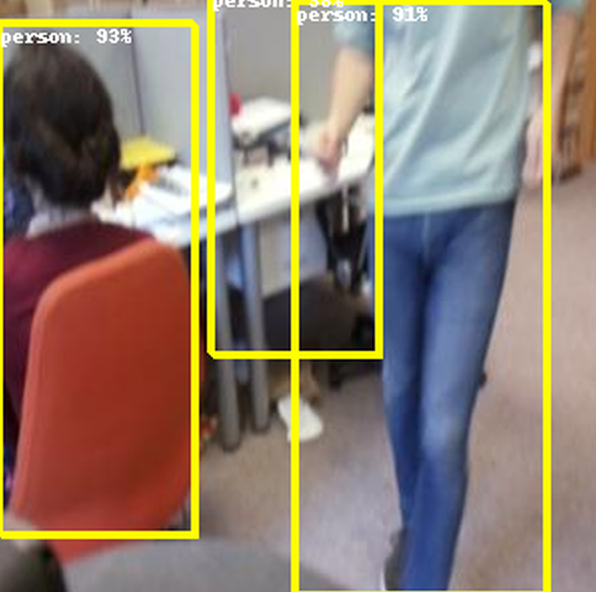
\includegraphics[width=0.5\textwidth]{methodology/box_around_people_hard}
  \caption{{\label{fig:box_around_people_hard}A photo of a person sitting and the bottom two thirds of another person standing, correctly predicted with 93\% and 91\% confidence respectively.}}
\end{figure}

Two people were correctly identified: a woman at a desk in the left of the frame with a confidence of 93\%, and the bottom two thirds of the author on the right side with a confidence of 91\%. Faces have been one of the easiest things to detect in computer vision \cite{website:face_detection_survey}, so it was a pleasant surprise to find that the network doesn't need a face at all.

There was also a false-positive detection in the centre of the frame. However, the confidence for this detection was 38\% - low enough that the recommended confidence threshold of 70\% confidence \cite{website:chuanqi305_nn_github} would have resulted in it being ignored.% \\

\subsection{Observed performance increase due to NCS}\label{ssec:meth_nn_performance_increase}
Next, the performance increase of the NCS was tested to confirm that the device was in fact necessary. For the purposes of the tests, the pre-processing time and latency of the camera were ignored as they are common to all methods of inferencing. It is worth noting that there will always be variability when timing the runtime of a process on a non-realtime OS using a language which occasionally pauses for garbage collection.

First, the Pi was tested on its own. Using the CPU, roughly a full second was required to get from pre-processed image to serialized results. Due to multithreading, up to four images may be processed side by side (staggered 250ms apart) for a total sampling rate of 4 Hz with a latency of 1 second.

Next, the Pi was tested with the Movidius NCS. It took around 20 ms to send the image to the devices memory, and then around 80ms to receive the result. The NCS can't process multiple images simultaneously, so this equated to a speed of 10 Hz with a latency of 100ms.

This proved that, short of using another form of CNN acceleration, the NCS was vital to the project's success.

